\documentclass[tikz, border=2pt]{standalone}

\usepackage{amsmath,amssymb}
\usepackage{pgfplots}
\pgfplotsset{compat=1.18}
\usepackage{xcolor}

\definecolor{utnblue}{RGB}{0, 51, 102}
\definecolor{utnred}{RGB}{204, 0, 0}

\begin{document}
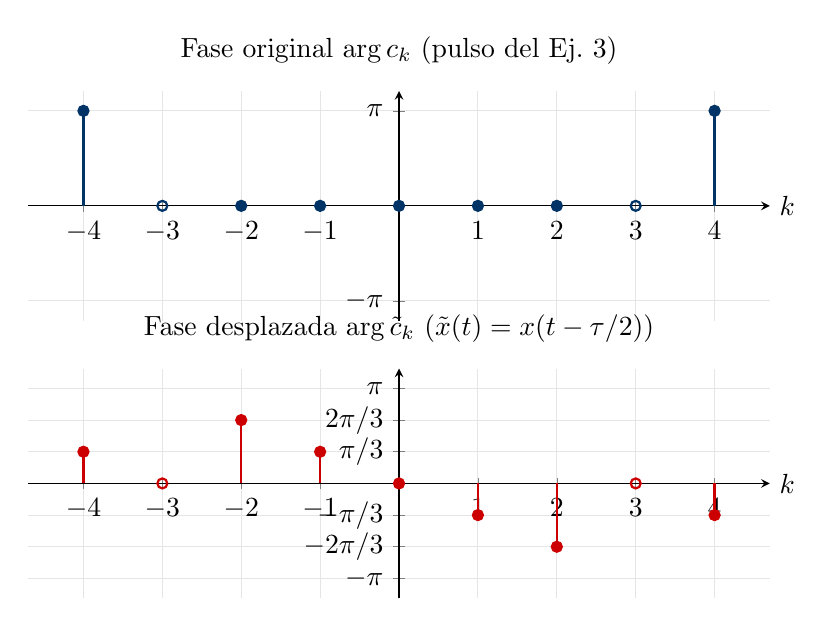
\begin{tikzpicture}

% --- Panel superior: fase original (Ej. 3) ---
\begin{axis}[
    name=orig,
    width=11cm, height=4.5cm,
    title={Fase original $\arg c_k$ (pulso del Ej.~3)},
    xmin=-4.7, xmax=4.7,
    ymin=-3.8, ymax=3.8,
    xtick={-4,-3,-2,-1,0,1,2,3,4},
    ytick={-3.1416, 0, 3.1416},
    yticklabels={$-\pi$, $0$, $\pi$},
    xlabel={$k$},
    axis lines=middle,
    enlargelimits=false,
    grid=major,
    grid style={gray!20},
    every axis x label/.style={at={(ticklabel* cs:1)}, anchor=west},
]
\addplot+[utnblue, thick, ycomb, mark=*, mark options={fill=utnblue, scale=0.9}]
    coordinates {(-4,3.1416) (-2,0) (-1,0) (0,0) (1,0) (2,0) (4,3.1416)};
\addplot[utnblue, mark=o, mark options={scale=0.9, line width=0.8pt}, only marks]
    coordinates {(-3,0) (3,0)};
\end{axis}

% --- Panel inferior: fase desplazada ---
\begin{axis}[
    at={(orig.below south west)}, anchor=north west, yshift=-0.6cm,
    width=11cm, height=4.5cm,
    title={Fase desplazada $\arg \tilde c_k$ ($\tilde x(t) = x(t - \tau/2)$)},
    xmin=-4.7, xmax=4.7,
    ymin=-3.8, ymax=3.8,
    xtick={-4,-3,-2,-1,0,1,2,3,4},
    ytick={-3.1416, -2.0944, -1.0472, 0, 1.0472, 2.0944, 3.1416},
    yticklabels={$-\pi$, $-2\pi/3$, $-\pi/3$, $0$, $\pi/3$, $2\pi/3$, $\pi$},
    xlabel={$k$},
    axis lines=middle,
    enlargelimits=false,
    grid=major,
    grid style={gray!20},
    every axis x label/.style={at={(ticklabel* cs:1)}, anchor=west},
]
\addplot+[utnred, thick, ycomb, mark=*, mark options={fill=utnred, scale=0.9}]
    coordinates {
        (-4, 1.0472) (-2, 2.0944) (-1, 1.0472) (0, 0) (1, -1.0472) (2, -2.0944) (4, -1.0472)
    };
\addplot[utnred, mark=o, mark options={scale=0.9, line width=0.8pt}, only marks]
    coordinates {(-3, 0) (3, 0)};
\end{axis}

\end{tikzpicture}
\end{document}
